This section will contain a brief overview of the progress over the past 4 weeks. A summary of each researched subject is given. The full details are provided further in this report. Added sections are marked in \add{blue}. The text in black has been added with respect to the comments I received last time, but does contain major adjustments. The progress section concludes with the planning of the next weeks.


\section{Finished subjects}

\subsection{Input mapping}

The input mapping describes the transformation of physical inputs to model inputs. The physical set-up has two inputs which can pressurize each bellow individually. However, the dynamic model is based on forces and moments. Hence, we seek to find $p \mapsto F$. This mapping has been found by using the $\verb+Abaqus+$ finite element program. It has been shown that pressurizing both bellows equally, will result in the same deformation as attaching a force to the top of the actuator. Therefore a mapping between force and pressure can be found, by comparing the elongation.


\subsection{Stiffness determination}

The input mapping allows to determine the elongation stiffness $K_\epsilon$ and curvature stiffness $K_\kappa$. An inverse kinematic solver was made. This model is able to obtain elongation and curvature from the FEM simulations. The elongation and curvature were approximated using the constant curvature approach. The hyper-elastic stiffness model as formulated in \cite{Caasenbrood2020StiffnessModel} was used. This resulted in the following results,


\begin{figure}[H]
    \centering
\begin{minipage}{0.5\textwidth}
        \centering
        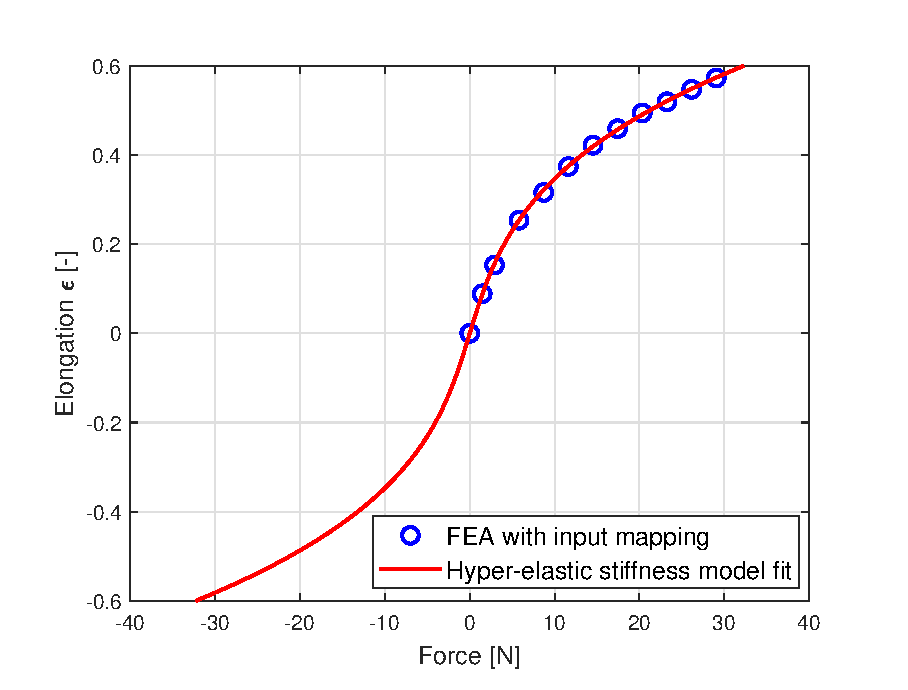
\includegraphics[width=\textwidth]{Figures/Chapter3/mappedforcevselongation.eps}
        \caption{Fitted stiffness model for elongation.}
    \end{minipage}\hfill
    \begin{minipage}{0.5\textwidth}
        \centering
        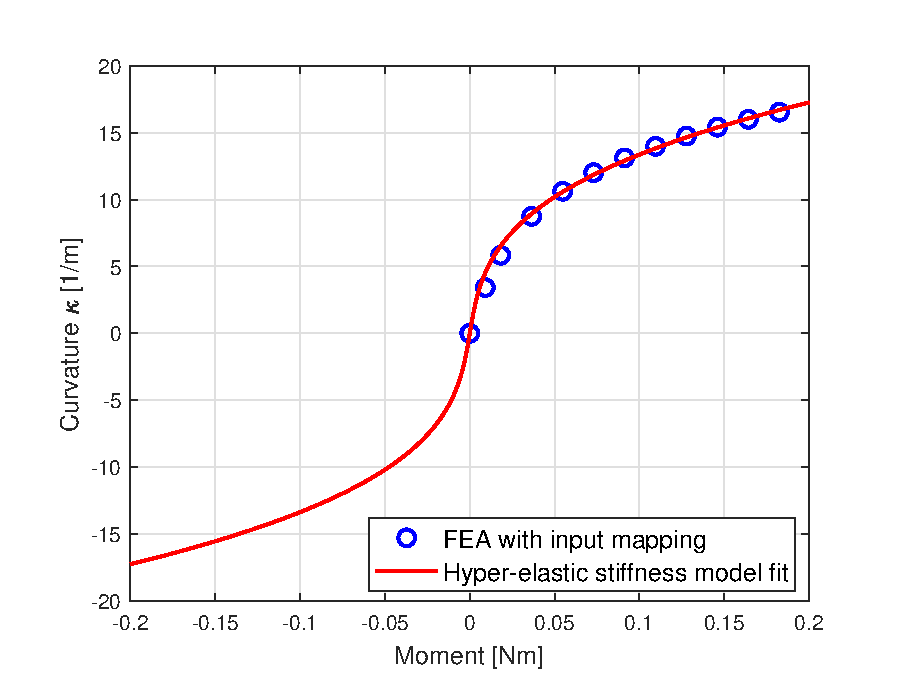
\includegraphics[width=\textwidth]{Figures/Chapter3/mappedmomentvscurvature.eps} 
        \caption{Fitted stiffness model for curvature.}
    \end{minipage}
\end{figure}


\section{Current research}

Now the non-linear stiffness has been obtained a start can be made with controller design. First a simplified non-linear model will be made in Matlab. This is done in Matlab since this is an environment I am more comfortable working with. After a controller has been found that is deemed good. I start implementation in C++.

The current research starts by implementing a forward dynamic model. First non-linear stiffness matrix $K$ is added. For now, mass matrix $M$ and damping matrix $D$ are constant, which gives,

\begin{equation}
    M = \begin{bmatrix} 0.0177 & 0 \\ 0 & 1.21e-5 \end{bmatrix}  ,  \hspace{20pt}  D = \begin{bmatrix} 0.1 & 0 \\ 0 & 0.02 \end{bmatrix} 
\end{equation}

where $M = \text{diag}(m, J_{xx})$ and $D = \text{diag}(d_\epsilon,d_\kappa)$. The mass matrix has been determined with $\verb+Abaqus+$. The damping matrix is arbitrary for now. With the previous found input mapping $H$, the system can be described by,

\begin{equation}
    M\Ddot{q} + C\dot{q} + K(q)q = Hp.
\end{equation}

Above can be rewritten to a system of first order differential equations using the state space formulation as,


\begin{equation}
     \begin{bmatrix} \dot{x_1} \\ \dot{x_2} \\\dot{x_3}  \\ \dot{x_4}  \end{bmatrix}   =      \begin{bmatrix} O_2 & I_2 \\ -M^{-1}K(q)  & -M^{-1}D \end{bmatrix}      \begin{bmatrix} x_1\\ x_2 \\x_3\\ x_4 \end{bmatrix}  +      \begin{bmatrix} O_2 \\ M^{-1}H   \end{bmatrix}       \begin{bmatrix} p_1\\ p_2   \end{bmatrix} 
\end{equation}

where $x = [\epsilon \hspace{4pt} \kappa \hspace{4pt} \dot{\epsilon} \hspace{4pt} \dot{\kappa}]^\top$.



Using $\verb+ode45.m+$ this state-space can be solved. First an initial condition should be given as,

\begin{equation}
    x_0 = [\epsilon_0 \hspace{4pt} \kappa_0 \hspace{4pt} \dot{\epsilon_0} \hspace{4pt} \dot{\kappa_0}] 
\end{equation}


it must be noted that $\kappa = \kappa_0  \hspace{4pt}  \forall  \hspace{4pt}  t $, when $\dot{\kappa_0} = 0 $ no matter what input is given. Define, $\theta$ as the rotation of the top plate. For $p_1  = p_2$ this will result in a 0 degrees rotation of top plate. For $p_1 \neq p_2 $ there will always be a rotation. Reason for this is the implementation of $\theta = \kappa L_0 \epsilon = q_2 L_0 q_1$ as $ q_1 \mapsto 0 $ for $t \mapsto \infty$. Figure \ref{fig:prob1_6_2} shows the result for $x_0 = [0.1 0.028 0 0]$. As can be seen $\dot{\kappa_0} = 0$ thus $\kappa$ this will be constant. In the figures below the input, so both pressures, are equal to 0. This can be seen as a "free" swing with an initial elongation of 20$\%$ and a top rotation of 10 degrees.  


\begin{figure}[H]
    \centering
    \begin{minipage}{.5\textwidth}
        \centering
        \includegraphics[width = \textwidth]{Figures/ProgresFigures/qp0.eps}
        \caption{Modal coordinates af function of $t$}
        \label{fig:prob1_6_2}
    \end{minipage}%
    \begin{minipage}{0.5\textwidth}
        \centering
        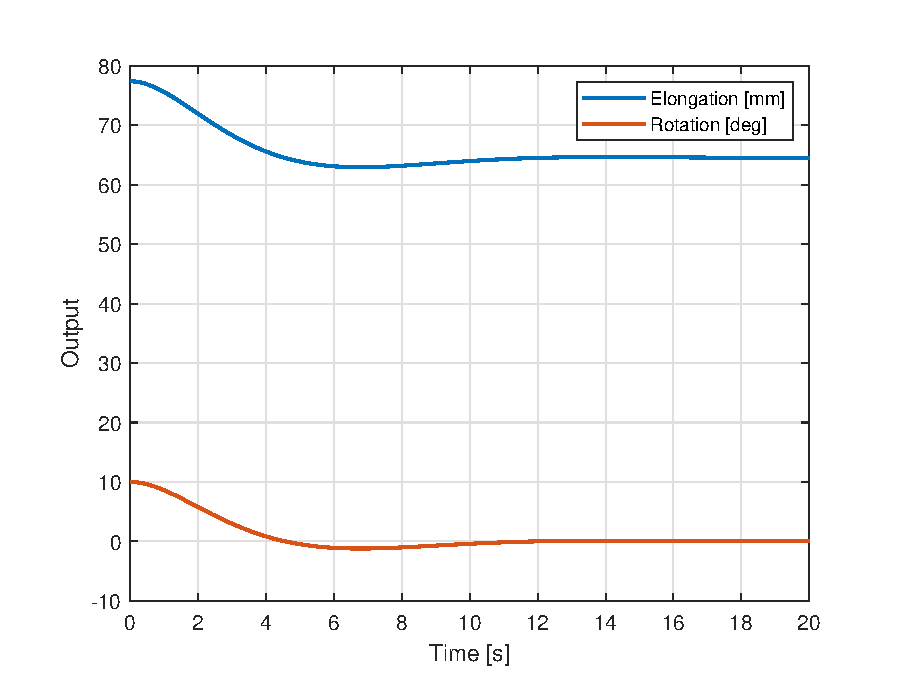
\includegraphics[width = \textwidth]{Figures/ProgresFigures/xp0.eps}
        \caption{Actuator length and rotation as function of $t$}
        \label{fig:prob1_6_1}
    \end{minipage}
\end{figure}


When making this report I discovered that there must be a bug somewhere in my script. It might have to do with the mass matrix being ill-conditioned since the inertia is so small. Or something else that I overlooked when writing this. Hopefully I will be able to fix this before the meeting tomorrow.












\textbf{Planning for coming weeks}


\begin{itemize}
    \item Implement non-linear stiffness in C++ code
    \item Correctly implement Matlab model with constant M and D matrices. This can be a good way of first controller design.
    \item Include gravity matrix in Matlab model
    \item Inverse current forward dynamic model in Matlab to an inverse dynamic analysis
    \item When a controller has been made, this can be implemented in C++ after which the first testing can take place.
\end{itemize}
